\chapter{Acoustic Perturbation Equations Solver}

\section{Synopsis}
The aim of APESolver is the prediction of aerodynamic sound generation. Through
the application of a splitting technique, the flow-induced acoustic field is
totally decoupled from the underlying incompressible hydrodynamic field. The
acoustic perturbation equations proposed by Ewert and Shroeder are employed as
the governing equations of the acoustic field and they assure stable
aeroacoustic simulation due to the suppression of the term related to the
production of perturbed vorticity. These equations are similar to the linearised
perturbed compressible equations, but while in the original formulation the flow
decomposition is based on solenoidal vortical perturbations as well as
irrotational acoustic perturbations, in this case perturbations are assumed to
be exclusively of acoustic nature.

\begin{align*}
      \frac{\partial \rho'}{\partial t} 
        + (\mathbf{U}\cdot \nabla)\rho'+\rho_0(\nabla \cdot \mathbf{u}') &= 0 \\
      \frac{\partial \mathbf{u}'}{\partial t}
        +\nabla(\mathbf{u}' \cdot \mathbf{U})+\frac{1}{\rho_0}\nabla p' &= 0 \\
      \frac{\partial p'}{\partial t}
        +\nabla \cdot (\gamma P \mathbf{u}+p'\mathbf{U})&=-\frac{DP'}{Dt}
\end{align*}
where $\mathbf{U},P)$ represents the base flow, $(\mathbf{u}',p')$
the perturbations and $D/Dt$ the material derivative.
$P'=P-p_{\infty}$ is the acoustic source term with $p_\infty$ is
the pressure at a reference value.

\section{usage}
\begin{lstlisting}[style=BashInputStyle]
APESolver session.xml
\end{lstlisting}

\section{Session file configuration}

\subsection{Solver Info}
\begin{itemize}
\item \inltt{Eqtype} Specifies the equation to solve. This should be set to
\inltt{APE}.
\item \inltt{UpwindType}
\end{itemize}

\subsection{Parameters}
\begin{itemize}
\item \inltt{Rho0}: Density
\item \inltt{Gamma}: Ratio of specific heats
\item \inltt{Pinfinity}: Ambient pressure
\end{itemize}

\subsection{Functions}
\begin{itemize}
\item \inltt{BaseFlow}
\item \inltt{Source}
\item \inltt{InitialConditions}
\end{itemize}


\section{Examples}
\subsection{Aeroacoustic Wave Propagation}

In this section it is explained how to set up a simple simulation of
aeroacoustic using the APESolver in Nektar++. We will study the simple case of
the propagation of an acoustic wave in the simple case where the base flow is
$\mathbf{U}=0, P=p_{\infty}=10^6$. The geometry is very simple and
consists of $64$ square elements as shown in the following figure.

\begin{figure}
	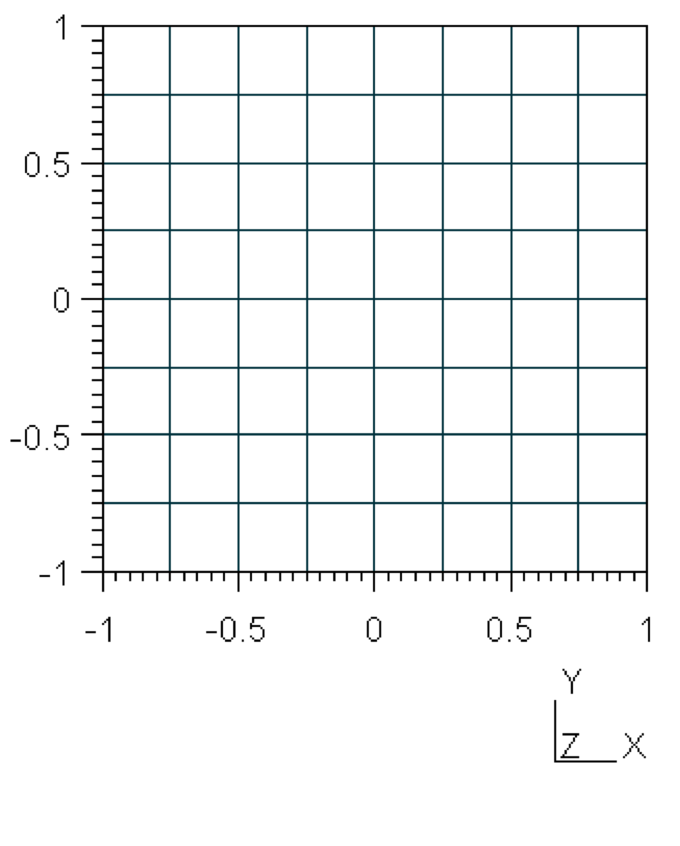
\includegraphics[width=300px]{Figures/APE_Geometry.png}
\end{figure}

Below it is possible to see how to set up the problem in the session file:

\begin{lstlisting}[style=XmlStyle]
<SOLVERINFO>
    <I PROPERTY="EQType" VALUE="APE"/> 
    <I PROPERTY="Projection" VALUE="DisContinuous"/>
    <I PROPERTY="TimeIntegrationMethod"  VALUE="ClassicalRungeKutta4"/>
    <I PROPERTY="UpwindType"  VALUE="Upwind"/> 
</SOLVERINFO>

<PARAMETERS>
    <P> TimeStep       = 0.00001             </P>
    <P> NumSteps       = 150                 </P>
    <P> FinTime        = TimeStep*NumSteps   </P>
    <P> IO_CheckSteps  = 6000                </P>
    <P> IO_InfoSteps   = 100                 </P>
    <P> Rho0             = 1.204               </P> <!-- Incompressible density -->
    <P> Gamma            = 1.4                 </P> <!-- Ratio of specific heats -->
    <P> Pinfinity      = 100000              </P> <!-- Ambient pressure -->
</PARAMETERS>
\end{lstlisting}

Let us not that to solve efficiently this problem a discontinuous Garlerkin
approach was used, setting the flag \inltt{Projection} to \inltt{Discontinuous}
and then selecting the appropriate upwind scheme using \inltt{UpwindType}. The
system is excited via the initial conditions putting a Gaussian pulse for pulse
fluctuations.  Finally, it is necessary to specify the base flow and the
eventual source terms using the following functions:

\begin{lstlisting}[style=XmlStyle]
<FUNCTION NAME="Baseflow"> 
    <E VAR="U0" VALUE="0" />
    <E VAR="V0" VALUE="0" />
    <E VAR="P0" VALUE="Pinfinity" />
</FUNCTION>

<FUNCTION NAME="Source"> 
    <E VAR="S"  VALUE="0" />
</FUNCTION>

<FUNCTION NAME="InitialConditions">
    <E VAR="p" VALUE="100*exp(-32*(((x)*(x))+((y)*(y))))" /> <!-- Gaussian pulse located at the origin -->
    <E VAR="u" VALUE="0" />
    <E VAR="v" VALUE="0" />
</FUNCTION>
\end{lstlisting}

It is the possible to launch the simulation typing:

\begin{lstlisting}[style=BashInputStyle]
APESolver Test_pulse.xml
\end{lstlisting}

In the following figure it is shown the pressure profile at different time
steps, showing the acoustic propagation:

\begin{figure}
	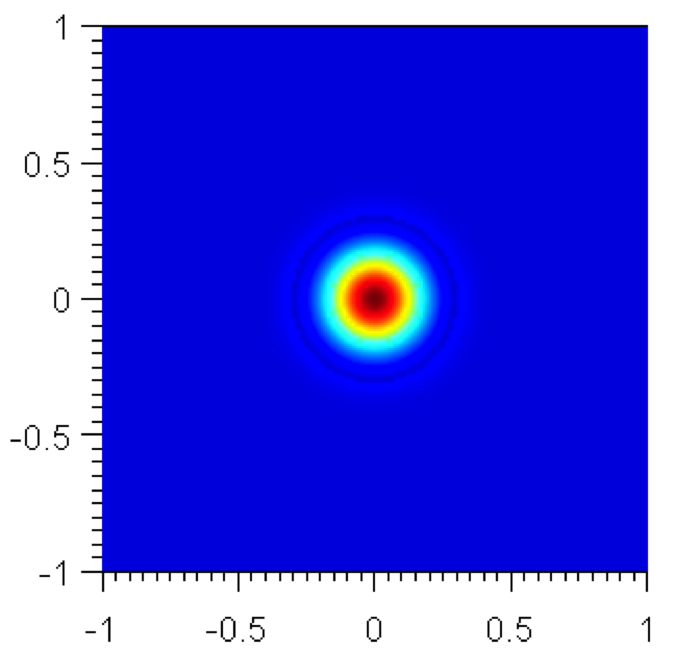
\includegraphics{Figures/Prop_1.png}
	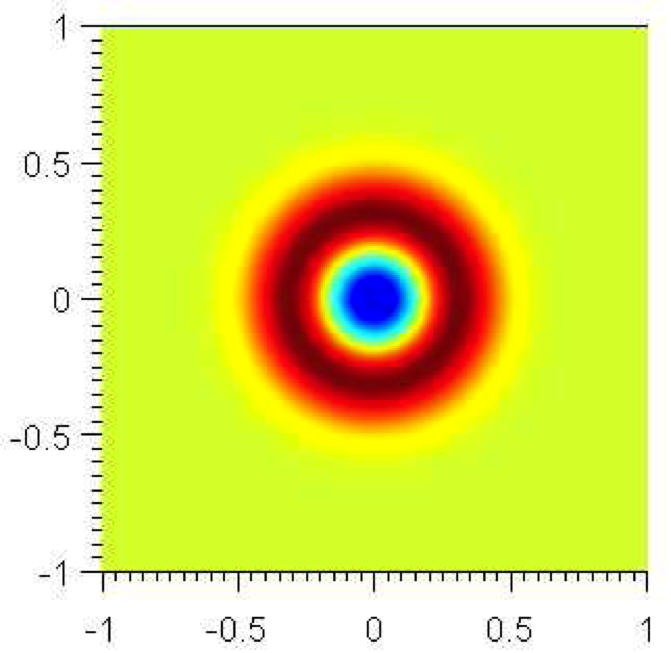
\includegraphics{Figures/Prop_2.png}
	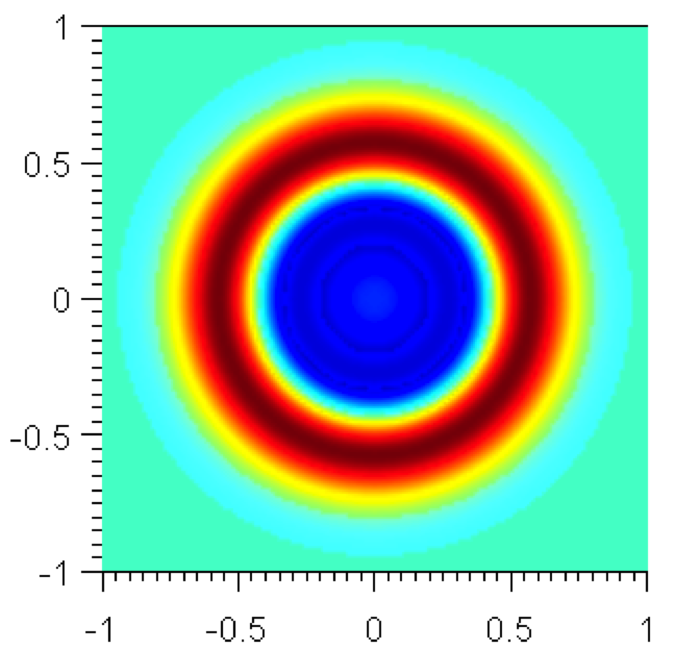
\includegraphics{Figures/Prop_3.png}
\end{figure}

It is possible to show the profile of the pressure perturbations with respect to
the spatial coordinate. The pressure fluctuations, that are concentrated  in a
specific locations at the beginning (as specified by the initial conditions),
propagate with time and for sufficiently large time the decay is exponential as
predicted by literature \cite{DoFf83}.

\begin{figure}
	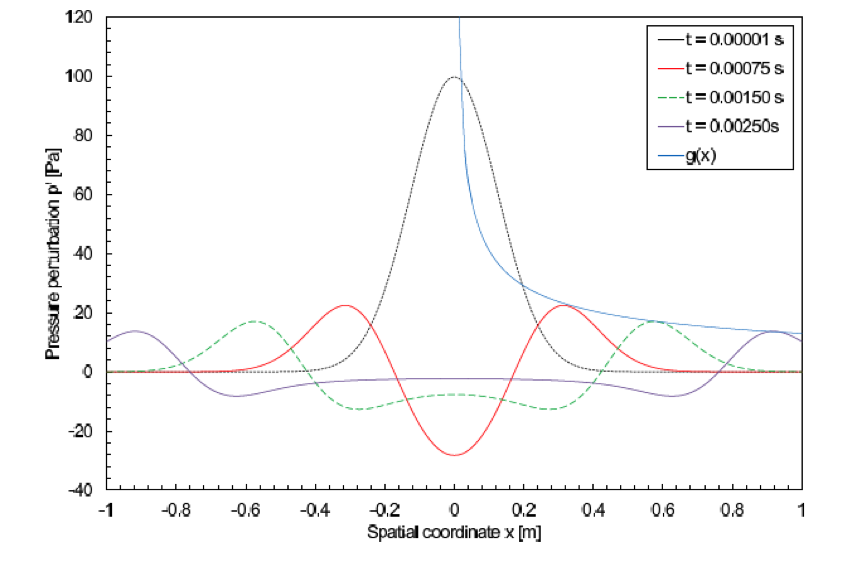
\includegraphics{Figures/prog_4.png}
\end{figure}

